\subsection{Times Table} % (fold)
\label{sub:times_table_flow}

This program prints out the times table for a number entered by the user, displaying from 1 x n to 10 x n. The description of the program is in Table \ref{tbl:flow-times-table}, the pseudocode in Listing \ref{lst:flow-times-pseudo}, the C code in Listing \ref{lst:flow-times-c}, and the Pascal code in Listing \ref{lst:flow-times-pas}.

\begin{table}[h]
\centering
\begin{tabular}{l|p{10cm}}
  \hline
  \multicolumn{2}{c}{\textbf{Program Description}} \\
  \hline
  \textbf{Name} & \emph{Times Table} \\
  \\
  \textbf{Description} & Displays the Times Table from 1 x n to 10 x n. \\
  \hline
\end{tabular}
\caption{Description of the Times Table program}
\label{tbl:flow-times-table}
\end{table}

\pseudocode{lst:flow-times-pseudo}{Pseudocode for Times Table program.}{./topics/control-flow/examples/times-table.txt}

\mynote{
This is an updated version of the Seven Times Table Program. See \sref{sub:times_table} \nameref{sub:times_table}.
}

\clearpage

\csection{\ccode{lst:flow-times-c}{C Times Table}{topics/control-flow/examples/times_table.c}}

\passection{\pascode{lst:flow-times-pas}{Pascal Times Table}{topics/control-flow/examples/TimesTable.pas}}

% subsection times_table (end)

\clearpage
\subsection{Circle Area} % (fold)
\label{sub:circle_area_control_flow}

This program prints out the area of a circle. The description of the program is in Table \ref{tbl:flow-circle-area}, the pseudocode in Listing \ref{lst:flow-circle-areas-pseudo}, the C code in Listing \ref{lst:flow-circle-areas-c}, and the Pascal code in Listing \ref{lst:flow-circle-areas-pas}.

\begin{table}[h]
\centering
\begin{tabular}{l|p{10cm}}
  \hline
  \multicolumn{2}{c}{\textbf{Program Description}} \\
  \hline
  \textbf{Name} & \emph{Circle Areas} \\
  \\
  \textbf{Description} & Displays the Circle Areas for circles with radius from 1.0 to 5.0 with increments of 0.1. \\
  \hline
\end{tabular}
\caption{Description of the Circle Areas program}
\label{tbl:flow-circle-area}
\end{table}

\pseudocode{lst:flow-circle-areas-pseudo}{Pseudocode for Circle Areas program.}{./topics/control-flow/examples/circle_areas.txt}

\mynote{
This is an updated version of the Circle Areas Program. See Section \ref{sub:circle_area_data} \nameref{sub:circle_area_data}.
}


\clearpage

\csection{\ccode{lst:flow-circle-areas-c}{C Circle Areas}{topics/control-flow/examples/circle_areas.c}}

\passection{\pascode{lst:flow-circle-areas-pas}{Pascal Circle Areas}{topics/control-flow/examples/CircleAreas.pas}}

% subsection circle_area (end)

\clearpage
\subsection{Moving Rectangle} % (fold)
\label{sub:moving_rectangle}

This example SwinGame code will move a rectangle back and forth across the screen.

\begin{table}[h]
\centering
\begin{tabular}{l|p{10cm}}
  \hline
  \multicolumn{2}{c}{\textbf{Program Description}} \\
  \hline
  \textbf{Name} & \emph{Moving Rectangle} \\
  \\
  \textbf{Description} & Displays a rectangle that is moved back and forth across the screen. \\
  \hline
\end{tabular}
\caption{Description of the Moving Rectangle program}
\label{tbl:flow-moving-rect}
\end{table}

\begin{figure}[h]
   \centering
   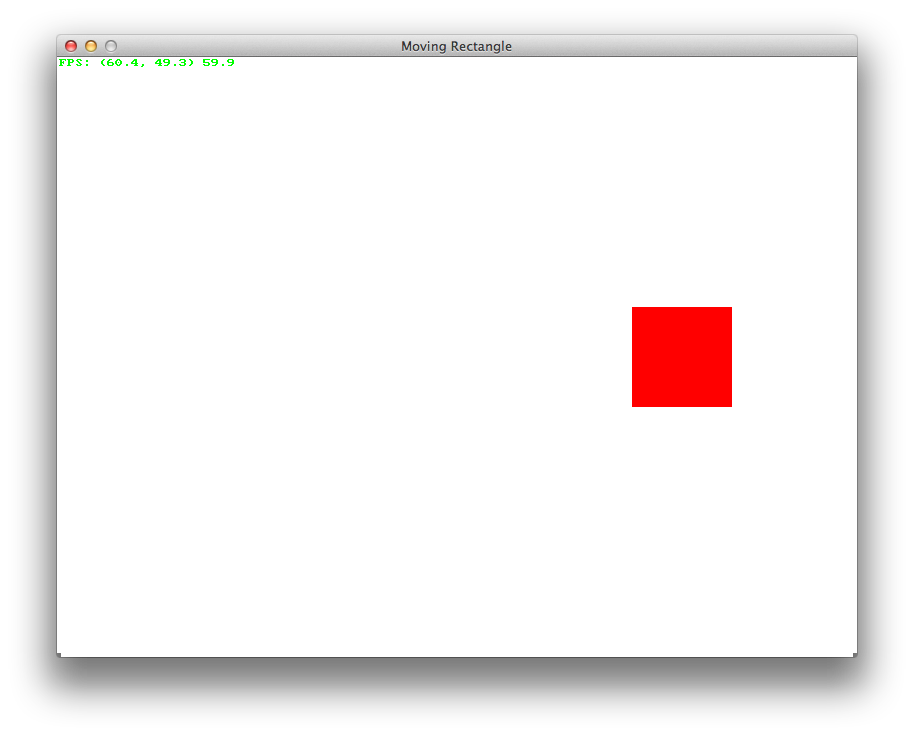
\includegraphics[width=0.8\textwidth]{./topics/control-flow/examples/MovingRect.png} 
   \caption{Example execution of the Moving Rectangle program}
   \label{fig:moving-rect-img}
\end{figure}


\clearpage

\cppsection{\ccode{clst:moving-rect}{C++ Moving Rect SwinGame code}{topics/control-flow/examples/moving-rect.cpp}}  

\passection{\pascode{plst:moving-rect}{Pascal Moving Rect SwinGame code}{topics/control-flow/examples/MovingRect.pas}}  


% subsection moving_rectangle (end)

\clearpage
\subsection{Button Click in SwinGame} % (fold)
\label{sub:button_click_in_swingame}

This example SwinGame code draws a rectangle that the user can `click'.

\begin{table}[h]
\centering
\begin{tabular}{l|p{10cm}}
  \hline
  \multicolumn{2}{c}{\textbf{Program Description}} \\
  \hline
  \textbf{Name} & \emph{Button Click} \\
  \\
  \textbf{Description} & Displays a rectangle the user can `click'. Having the mouse held down over the rectangle changes it to a filled rectangle. Clicking the rectangle shows the text `Clicked' in the top left corner. \\
  \hline
\end{tabular}
\caption{Description of the Button Click program}
\label{tbl:flow-button-click}
\end{table}

\begin{figure}[h]
   \centering
   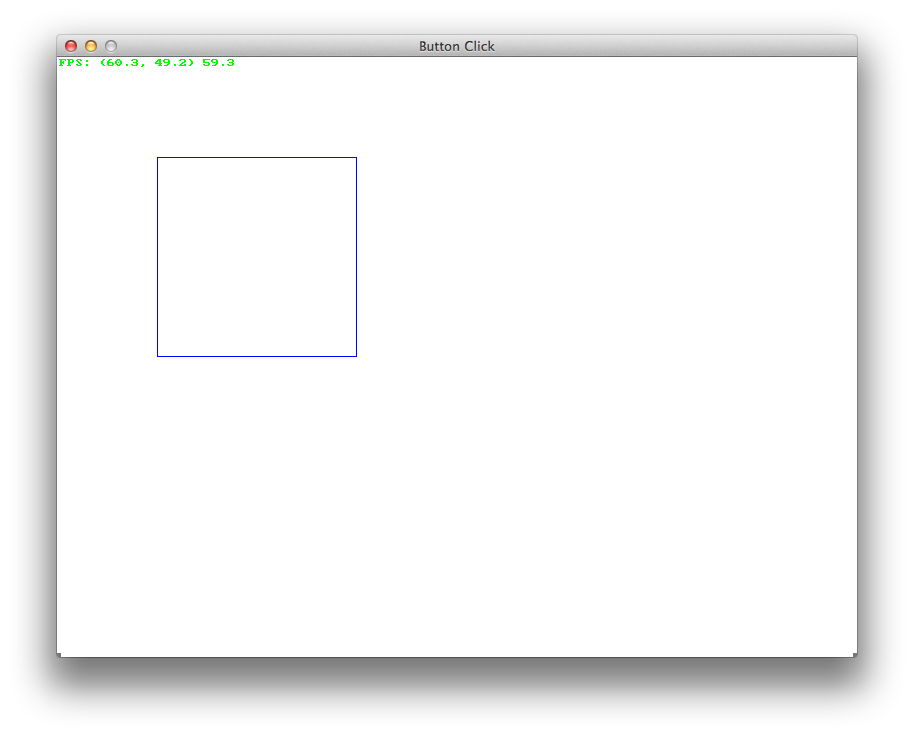
\includegraphics[width=0.8\textwidth]{./topics/control-flow/examples/ButtonClick.png} 
   \caption{Example execution of the Button Click program}
   \label{fig:button-click-img}
\end{figure}


\clearpage

\cppsection{\ccode{clst:swingame_button}{C++ Simple Button using SwinGame code}{topics/control-flow/examples/button-click.cpp}}  

\passection{\pascode{plst:button-click}{Pascal Button Click code}{topics/control-flow/examples/ButtonClick.pas}}  


% subsection button_click_in_swingame (end)

% \clearpage
% \subsection{Rocket Launch} % (fold)
% \label{sub:rocket_launch}
% 
% \cppsection{\ccode{clst:rocket_launch}{C++ Rocket Launch using SwinGame code (Continues in \lref{clst:rocket_launch1}) }{topics/control-flow/examples/rocket_launch.cpp}}
% 
% \begin{figure}[p]
%   \cppsection{\ccode{clst:rocket_launch1}{C++ Rocket Launch using SwinGame code (cont.) }{topics/control-flow/examples/rocket_launch1.cpp}}
% \end{figure}
% 
% \begin{figure}[p]
%   \cppsection{\ccode{clst:rocket_launch2}{C++ Rocket Launch using SwinGame code (cont.) }{topics/control-flow/examples/rocket_launch2.cpp}}
% \end{figure}
% 
% 
% % subsection rocket_launch (end)